\lecture{Fabbricati e Servizi di Stabilimento}{25~-~01~-~2026}
%
%
\section{Criteri di Scelta e Tipologie di Fabbricato}
La selezione del fabbricato industriale non è casuale ma deve rispondere a precisi requisiti economici e operativi. I principali criteri di scelta includono:
\begin{itemize}
    \item Le esigenze del \textbf{Plant Layout} (disposizione di macchinari e lavorazioni);
    \item I costi di costruzione, acquisto del terreno e gestione operativa (illuminazione, riscaldamento, ventilazione).
\end{itemize}
Si distinguono due macro-categorie di strutture:
\begin{enumerate}
    \item \textbf{Fabbricati a più piani}: utilizzati storicamente o per esigenze specifiche (es. ex stabilimento Fiat Lingotto \dots).
    \item \textbf{Fabbricati a un piano}: la tipologia più diffusa, caratterizzata da ampie superfici libere (es. capannoni prefabbricati \dots).
\end{enumerate}

%
\subsection{Caratteristiche Strutturali}
Per definire un fabbricato idoneo al layout produttivo, è fondamentale analizzare parametri geometrici e strutturali specifici:
\begin{itemize}
    \item \emph{La Maglia}: Definisce l'ossatura portante. È la distanza (interasse) tra i pilastri lungo l'asse longitudinale e trasversale. Maglie più ampie offrono maggiore flessibilità. Vedi figura \ref{fig:maglia}.
    \item \emph{Altezza netta sotto filo catena} (h.s.f.c.): È l'altezza libera tra il pavimento e il punto più basso della struttura di copertura. Le misure standard sono 6, 7 o 8 metri, ma nei magazzini automatici si superano i 15 metri. Vedi figura \ref{fig:altezza}.
    \item \emph{Suddivisione verticale}: In uno stabilimento moderno si individuano diversi livelli funzionali:
          \begin{itemize}
              \item \textbf{Livello -1}: Fondazioni e servizi interrati;
              \item \textbf{Livello 0}: Piano di lavoro (macchinari, transito uomini/mezzi);
              \item \textbf{Livello 1 e 2}: Trasporti aerei e distribuzione utenze (sopra i macchinari).
          \end{itemize}
\end{itemize}

\begin{figure}
    \centering
    \begin{subfigure}{0.45\linewidth}
        \centering
        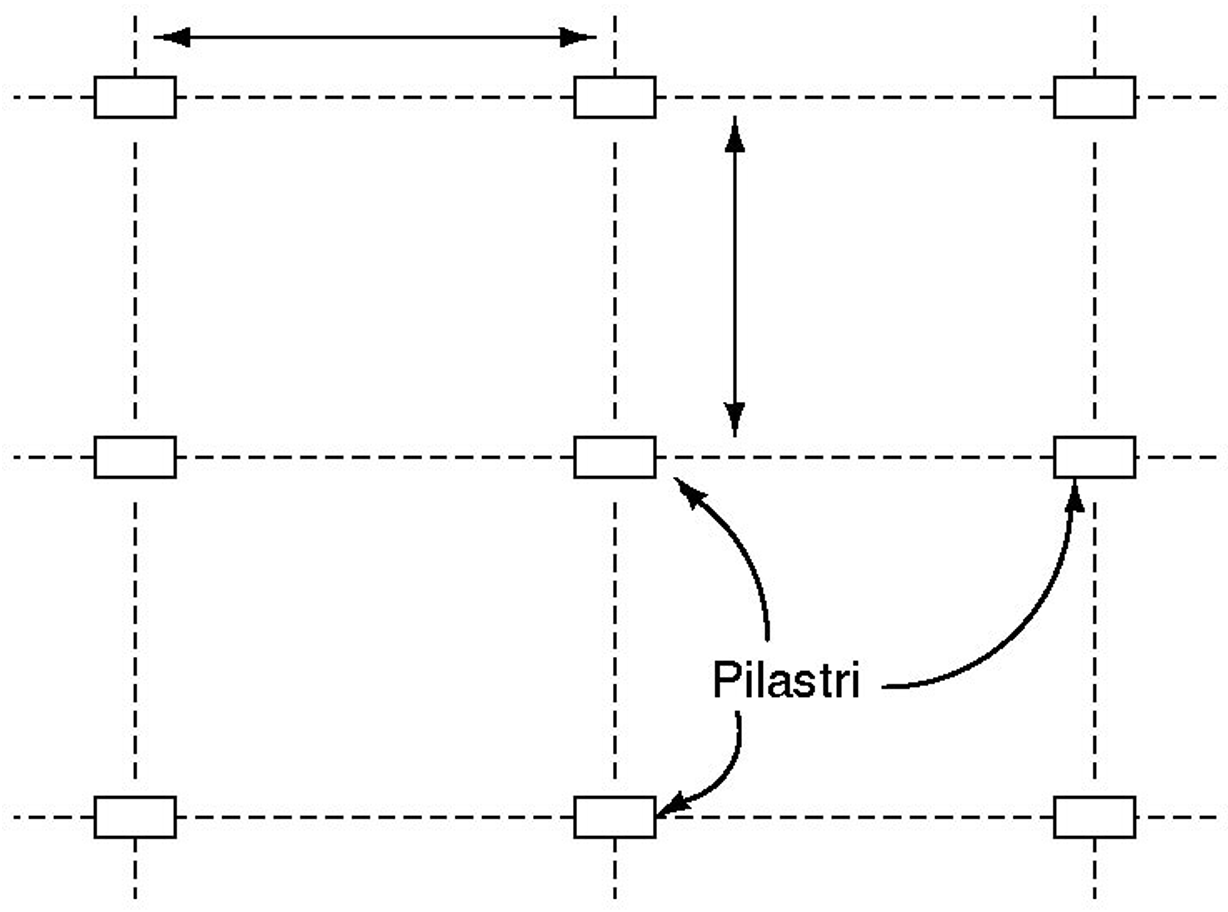
\includegraphics[width=\linewidth]{assets/Picture 10.png}
        \caption{Struttura portante di un frabbricato}\label{fig:maglia}
    \end{subfigure}
    \begin{subfigure}{0.45\linewidth}
        \centering
        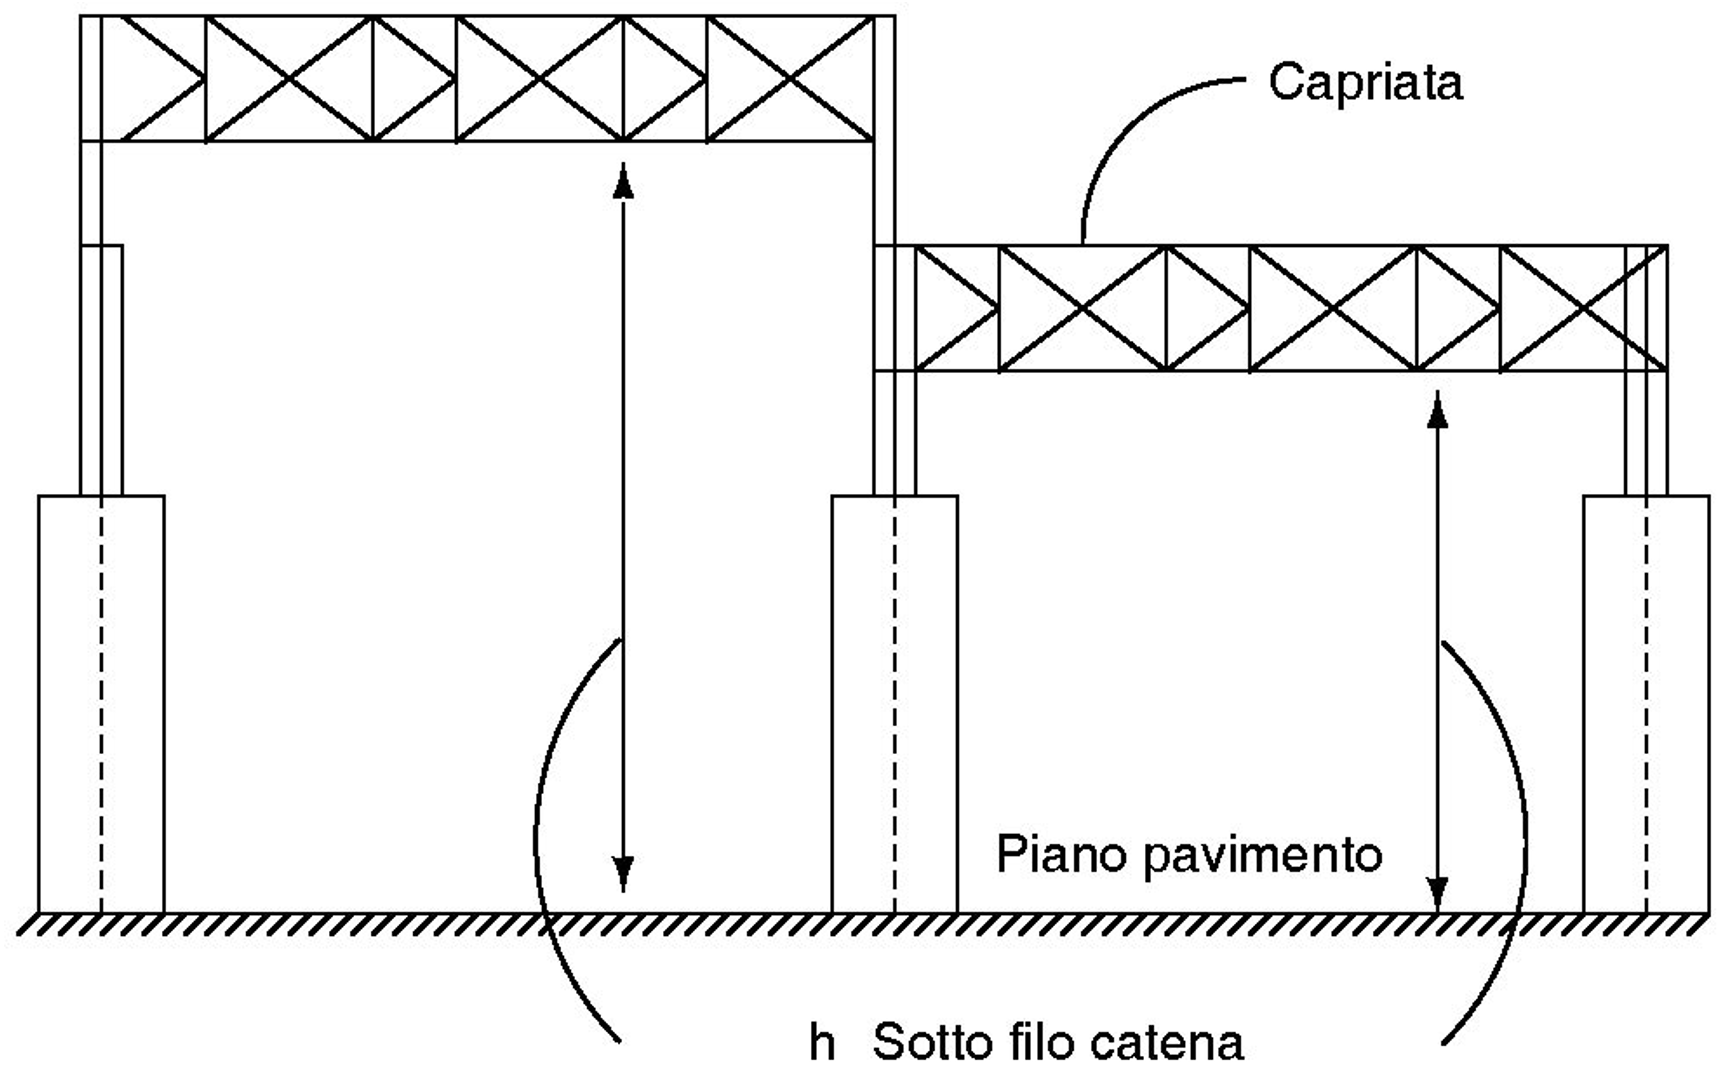
\includegraphics[width=\linewidth]{assets/Picture 111.png}
        \caption{Altezza netta sotto filo catena}\label{fig:altezza}
    \end{subfigure}
    \caption{Caratteristiche strutturali di un fabbricato}\label{fig:fabbricato}
\end{figure}

\subsubsection{Strutture Portanti}
La scelta del materiale strutturale influenza costi e prestazioni.
%
\paragraph{Cemento Armato e precompresso} Garantisce elevata resistenza al fuoco, non teme la corrosione, ha un'ottima inerzia termica e smorza rumori e vibrazioni. Le strutture precompresse permettono maglie ampie e montaggio rapido. Vedi figura \ref{fig:cemento_armato}.

Interassi (in metri) delle maglie più comunumente adottati sono:
\begin{itemize}
    \item $ 20 \times 12 $, $ 24 \times 12 $, $ 26 \times 14 $;
    \item Con valori massimi di $ 7.5 \times 35 $, $ 12 \times 34 $.
\end{itemize}

%
\paragraph{Acciaio} Vantaggioso per rapidità di costruzione, leggerezza e capacità di coprire grandi luci con forti sovraccarichi. Ha come svantaggi una bassa resistenza al fuoco e necessità di manutenzione contro la corrosione. Vedi figura \ref{fig:acciaio}.


Interassi (in metri) delle maglie più comunumente adottati sono:
\begin{itemize}
    \item $ 12 \times 12 $, $ 16 \times 16 $, $ 12 \times 16 $, $ 12 \times 24 $, $ 20 \times 20 $;
    \item Recentemente sono state realizzate strutture con maglie più ampie, ad esempio $ 12 \times 30 $, $ 12 \times 36 $, $ 14 \times 28 $.
\end{itemize}

\begin{figure}
    \centering
    \begin{subfigure}{0.45\linewidth}
        \centering
        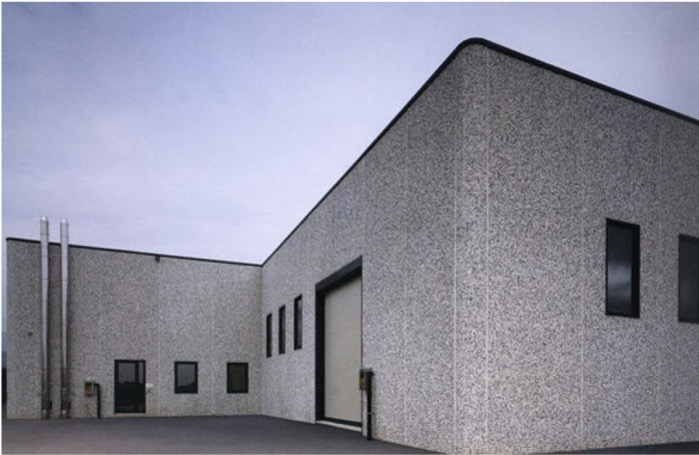
\includegraphics[width=\linewidth]{assets/Picture 8.jpg}
        \caption{Fabbricato in cemento armato}\label{fig:cemento_armato}
    \end{subfigure}
    \begin{subfigure}{0.39\linewidth}
        \centering
        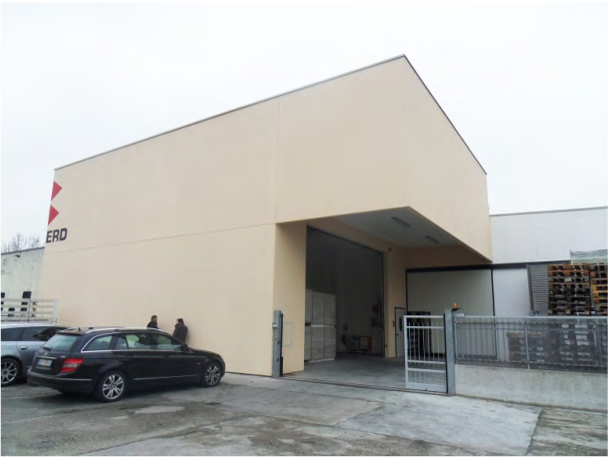
\includegraphics[width=\linewidth]{assets/Picture 9.png}
        \caption{Fabbricato in acciaio}\label{fig:acciaio}
    \end{subfigure}
    \caption{Fabbricati in cemento armato e acciaio}\label{fig:fabbricati}
\end{figure}

\subsubsection{Fondazioni}
Devono essere progettate in base al terreno (compatto o sciolto). Le fondazioni dei macchinari richiedono attenzione particolare: devono avere grande massa e supporti elastici/antivibranti per evitare la risonanza e la trasmissione di vibrazioni alla struttura.

%
\subsection{Elementi Architettonici}
\subsubsection{Coperture e Illuminazione}
%
\paragraph{Coperture} Le coperture devono assicurare impermeabilizzazione, isolamento e spesso anche illuminazione e ventilazione. Esistono diverse configurazioni:
\begin{itemize}
    \item Tetto a falde con finestrature a nastro o sul tetto;
    \item Tetto piano con lucernari (\emph{triangolari o semicircolari});
    \item Tetto a shed (\emph{denti di sega}): Tipico per l'illuminazione naturale diffusa.
\end{itemize}
%
\paragraph{Illuminazione} L'uso della luce naturale va integrato con quella artificiale per evitare abbagliamenti e garantire costanza.

Sono presenti dei requisiti di illuminazione (la cui unità è ``lux''):
\begin{itemize}
    \item Assemblaggio macchinario pesante: 200 lux;
    \item Assemblaggio veicoli: 300 lux;
    \item Uffici di progettazione ed elettronica: 500 lux;
    \item Oggetti di piccole dimensioni: 1000 lux.
\end{itemize}

\subsubsection{Pavimentazioni}
%
\paragraph{Pavimenti} Devono resistere a urti e vibrazioni, essere facili da pulire (antipolvere) ed economici.
%
\paragraph{Portoni} La tipologia dipende dall'uso. Si va dai portoni flessibili a strisce (per transiti veloci), a quelli a libro o scorrevoli, fino ai portoni sezionali e ad impacchettamento rapido. Per grandi aperture (es. hangar) si usano i ``Megadoors''. Vedi figura \ref{fig:portoni}.

\begin{figure}
    \centering
    \begin{subfigure}{0.45\linewidth}
        \centering
        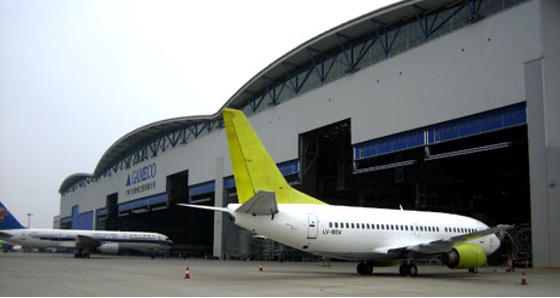
\includegraphics[width=\linewidth]{assets/Picture 12.jpg}
        \caption{Megadoor}\label{fig:megadoor}
    \end{subfigure}
    \begin{subfigure}{0.2\linewidth}
        \centering
        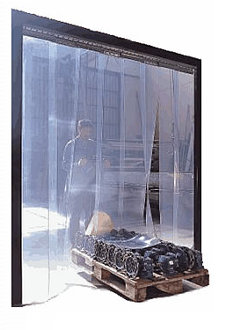
\includegraphics[width=\linewidth]{assets/Picture 13.png}
        \caption{Portone flessibile}\label{fig:portone_flessibile}
    \end{subfigure}
    \caption{Portoni industriali}\label{fig:portoni}
\end{figure}

%
\section{Servizi Generali di Stabilimento e Layout Interno}
La progettazione include aree accessorie fondamentali per il funzionamento dell'impianto.
%
\subsection{Uffici e corridoi}
%
\paragraph{Uffici}
Secondo la logica Lean, gli uffici di supervisione devono essere al centro dell'impianto (``nel mezzo dell'azione''), con pareti vetrate per la visibilità e aree comuni per la comunicazione.

%
\paragraph{Corridoi}
I corridoi devono essere rettilinei e separare, se possibile, pedoni e mezzi. I corridoi non devono avere ostacoli e possono essere a T, H, croce o a rete. Vedi figura \ref{fig:corridoi}.

Si suddividono in:
\begin{itemize}
    \item \textbf{Corridoi principali}: $ 4 \div 6 $ m;
    \item \textbf{Corridoi secondari}: $ 2 \div 4 $ m;
    \item \textbf{Passaggi uomo}: $ 0,70 \div 2,5 $ m.
\end{itemize}

\begin{figure}
    \centering
    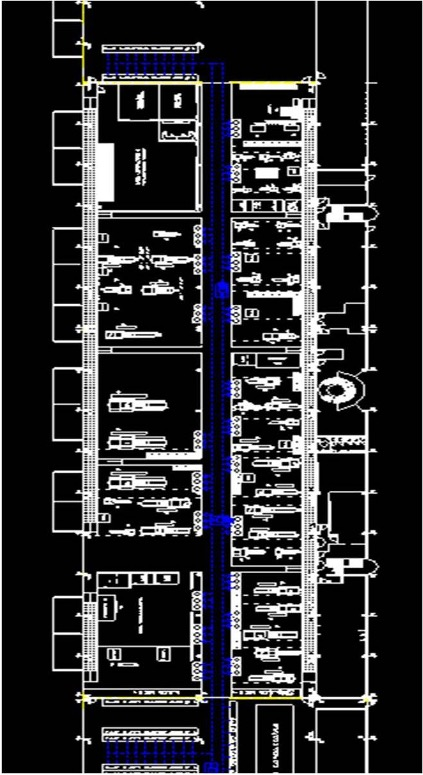
\includegraphics[width=0.3\linewidth, angle=270]{assets/Picture 14.jpg}
    \caption{Corridoi}\label{fig:corridoi}
\end{figure}

%
\subsection{Banchine di carico/scarico}
Le banchine velocizzano i flussi logistici e devono compensare il dislivello tra mezzo e magazzino. Possono essere disposte a pettine (inclinate) o ortogonali, spesso dotate di Dock-House esterne per non occupare spazio interno. Vedi figura \ref{fig:banchine}.

\begin{figure}
    \centering
    \begin{subfigure}{0.45\linewidth}
        \centering
        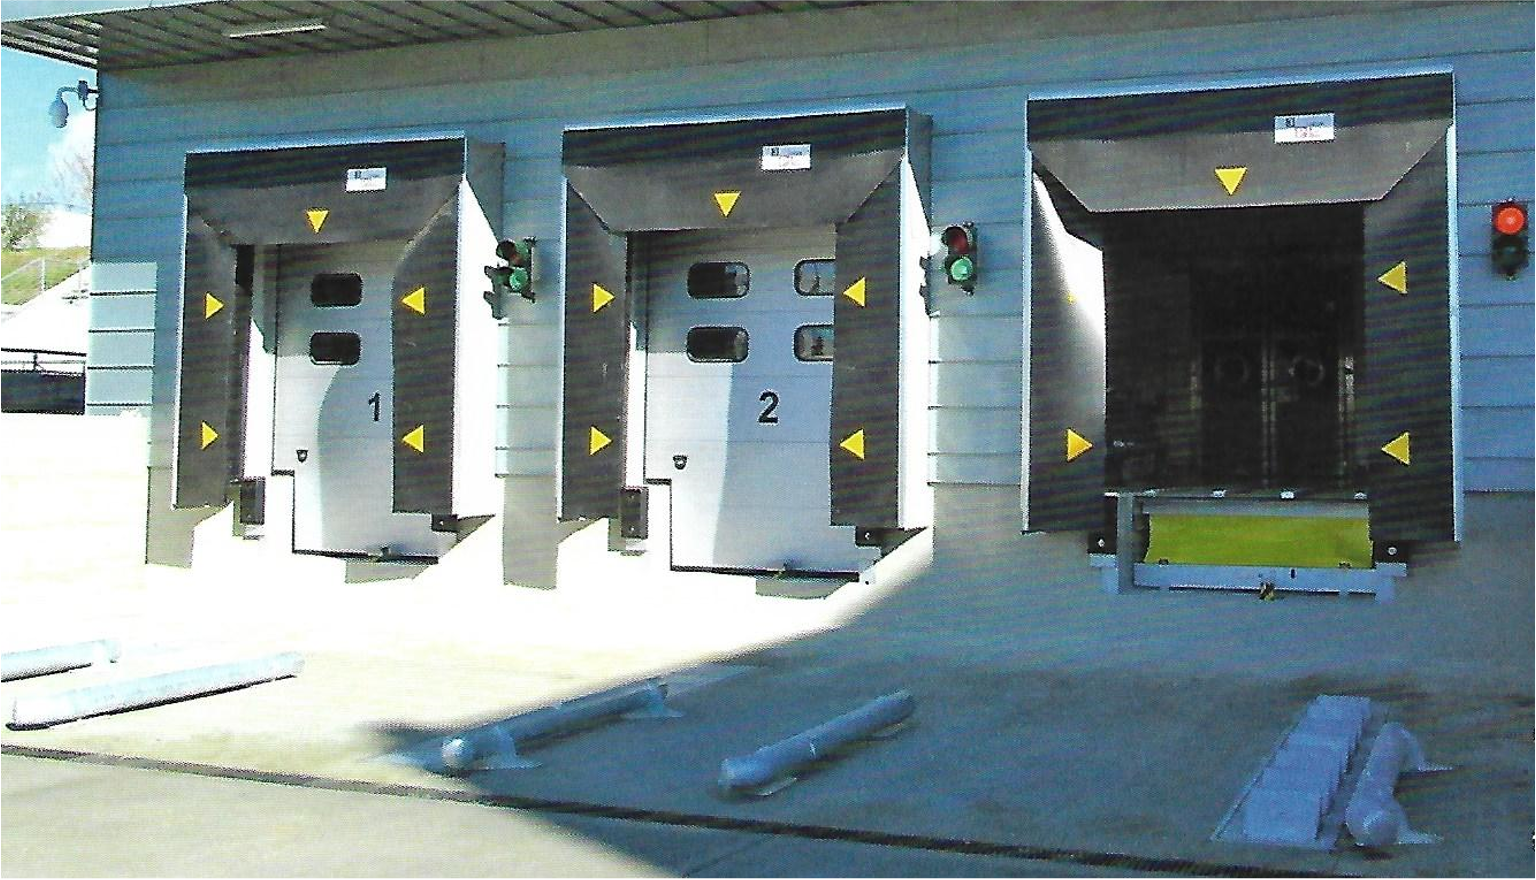
\includegraphics[width=\linewidth]{assets/15.png}
        \caption{Banchine}\label{fig:ban}
    \end{subfigure}
    \begin{subfigure}{0.3\linewidth}
        \centering
        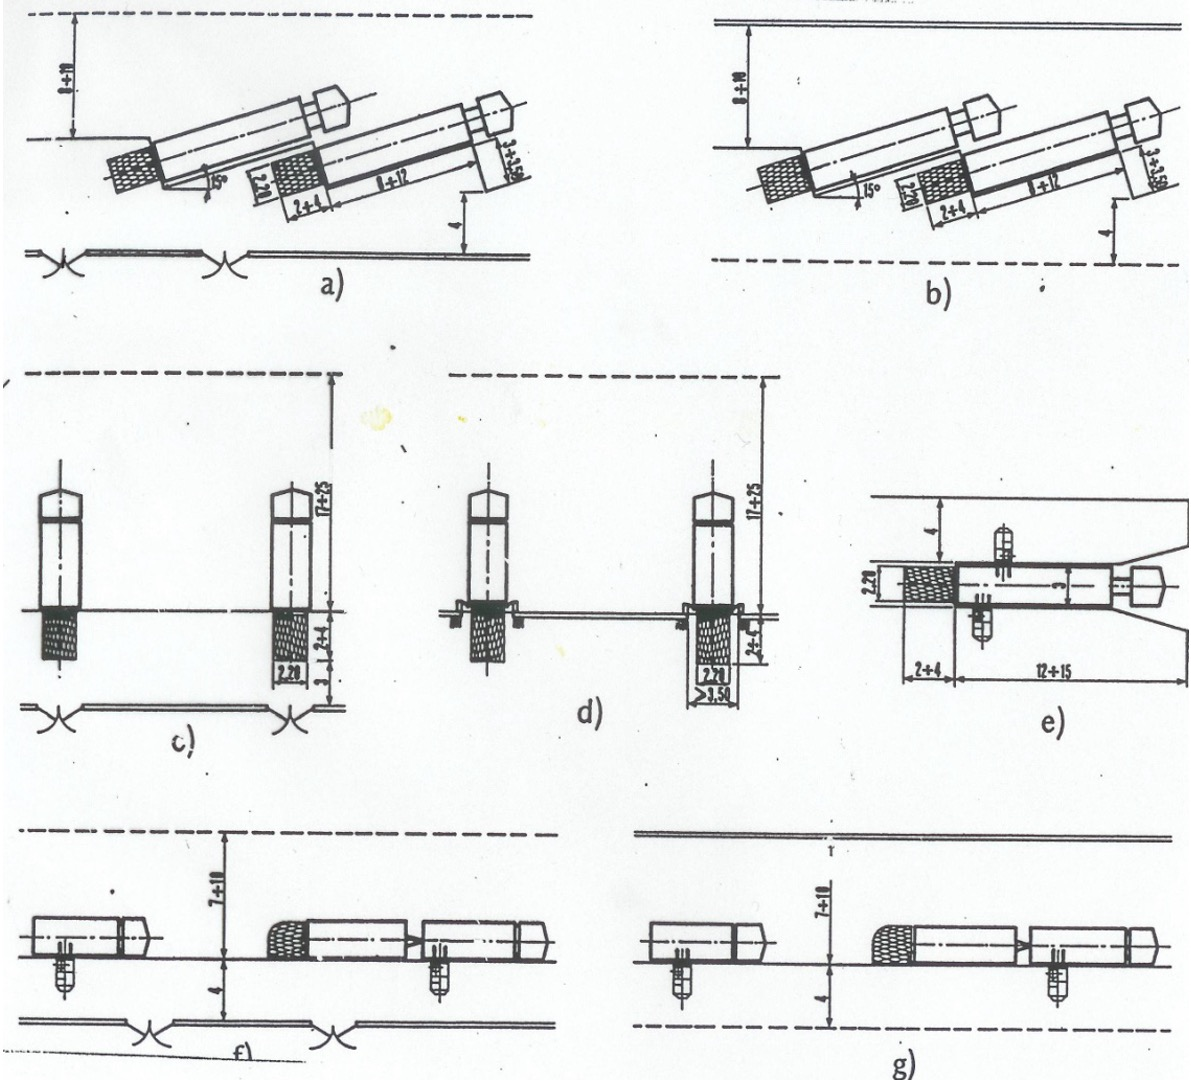
\includegraphics[width=\linewidth]{assets/16.jpg}
        \caption{Disposizione banchine}\label{fig:banchine_disposizione}
    \end{subfigure}
    \caption{Banchine di carico/scarico}\label{fig:banchine}
\end{figure}

%
\subsubsection{Dimensionamento}
%
\paragraph{Ricevimento merci}
\[
    N_{B} = M \cdot t_{S}
\]
Dove $ N_{B} $ è il numero di banchine, $ M $ tasso di arrivo di mezzi per unità di tempo, $ t_{S} $  tempo di scarico di un mezzo (ore).

%
\subparagraph{Area di ricevimento merci}
\[
    A_{R} = A \cdot Q \cdot t_{M}
\]
Dove $ A_{R} $ è l'area di ricevimento (m$ ^{2} $), $ A $ area di base dell'unità di carico (m$ ^{2} $), $ Q $ numero di unità di carico di materia prima in ingresso per unità di tempo (flusso in ingresso), $ t_{M} $ tempo di accettazione merce e di movimentazione verso magazzino materie prime.

%
\paragraph{Spedizione merci} Il numero di banchine dipende dal rapporto tra il \emph{volume di prodotto} e il \emph{volume del mezzo}:
\[
    N_{B} = \frac{V_{P}}{V_{M}}
\]
\begin{itemize}
    \item Volume di prodotto $ V_{P} $: quantità (in $ \text{m}^{3} $) di prodotto da spedire nel tempo necessario a caricare un mezzo;
    \item Volume del mezzo $ V_{M} $: 1 TEU ($ 34.5\ \text{m}^{3} $), 1 FEU ($ 63.4\ \text{m}^{3} $).
    \item Superficie totale: somma delle superfici necessarie per imballare, pesare e movimentare i prodotti, preparare i documenti di trasporto \dots
\end{itemize}
%
\subsection{Servizi per il Personale}
%
\paragraph{Parcheggi} Si stimano $0.4$ - $ 0.6 $ posti auto per dipendente, con un'area di $ 20 $ - $ 25 $ $\text{m}^2$ per posto.
Ogni 50 posti auto deve esserci un posto con larghezza $ 3.2 $ $ \text{m} $ per disabili.

Riguardo i parcheggi per moto/bici si ipotizza $ 0.1 $ - $ 0.15 $ posti per dipendente, con un'area di $ 2 $ - $ 5 $ $ \text{m}^2 $ per posto.

Le vie di accesso devono essere larghe:
\begin{itemize}
    \item $ 3.00\ \text{m} $ per flusso unidirezionale;
    \item $ 5.50\ \text{m} $ per flusso bidirezionale;
    \item Marciapiedi lungo il perimetro dello stabilimento: larghezza di $ 1 $ - $ 1.5 $ m.
\end{itemize}

%
\subsection{Isola tecnica}
Area dedicata alla generazione e distribuzione dei servomezzi (elettricità, aria compressa, acqua, HVAC), separata per sicurezza e gestione.

%
\section{Layout Generale P.R.G.}
Il Piano Regolatore Generale (P.R.G.) definisce la disposizione complessiva del sito industriale, includendo corpo di fabbrica principale, edifici secondari (uffici, mensa), viabilità, parcheggi, aree verdi e spazi per futuri ampliamenti. Vedi figura \ref{fig:prg}.
\begin{figure}
    \centering
    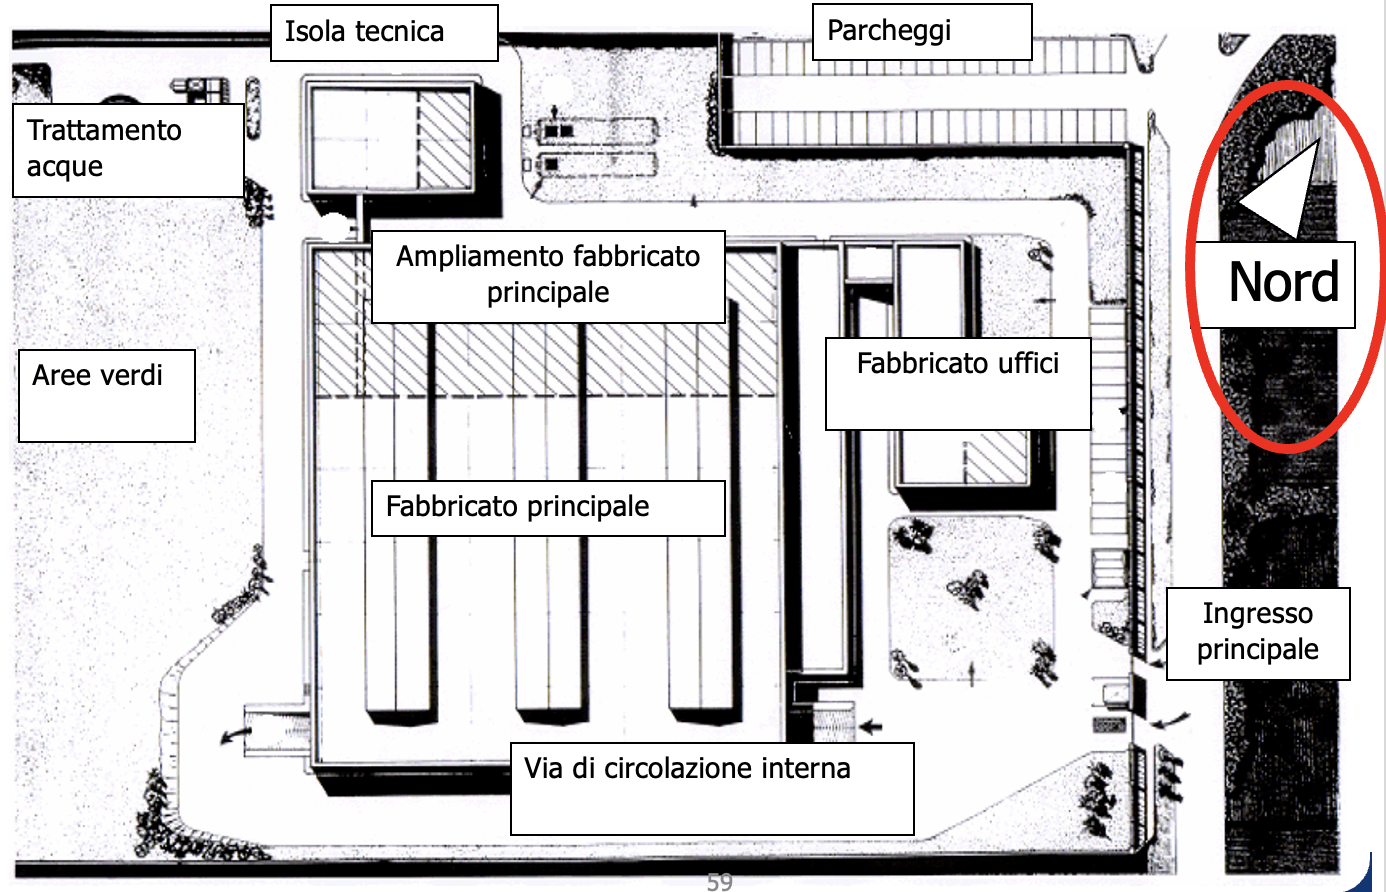
\includegraphics[width=0.6\linewidth]{assets/Screenshot 2026-01-25 at 18.03.31.png}
    \caption{Esempio di P.R.G.}\label{fig:prg}
\end{figure}

%
\section{Building Information Modelling (BIM)}
Il BIM è una metodologia basata su un modello digitale 3D interattivo che accompagna l'edificio lungo tutto il suo ciclo di vita (progettazione, costruzione, gestione).
%
\paragraph{Funzioni} Non è solo disegno 3D, ma un database che contiene specifiche tecniche, costi e tempi. Permette l'estrazione automatica di quantità (Quantity Take-Off), la stima dei costi e l'analisi delle prestazioni (energetiche, strutturali).

%
\paragraph{Vantaggi}
\begin{itemize}
    \item Migliore visualizzazione e risoluzione dei conflitti progettuali;
    \item Precisione: Stima dei costi con errore entro il 3\%;
    \item Velocità: Riduzione dei tempi di progetto fino al 7\%;
    \item Facility Management: I dati raccolti sono essenziali per la manutenzione futura.
\end{itemize}